\documentclass{article}
\usepackage[utf8]{inputenc}
\usepackage{hyperref}
\usepackage{graphicx}

\title{Lex \& Yacc}
\author{Sullivan PINEAU \and Sebastien VALLEE }
\date{April 2017}

\begin{document}

\maketitle

\section{Introduction}
    On a tous entendu parler un jour ou l'autre de lex et yacc, ne serait-ce que pour compiler certains logiciels ... Mais qu'est ce que c'est ?
    
    Lex et yacc sont un ensemble d'outils très utile si un programme C/C++ a recours à un fichier de données structurées et qu'il faut le parcourir, en vérifier sa validité, en extraire les données utiles etc... Lex et Yacc permettent de décrire la syntaxe du fichier (les mots clefs structurants) ainsi que sa grammaire (les enchaînements de mots clefs et l'exploitation des données parsées) dans un langage de haut niveau. Une fois ce travail accompli, ces deux outils génèrent une fonction C facilement intégrale dans un projet C/C++. 
    
\section{Lex}
    Lex est un analyseur lexical, c'est à dire que celui-ci permet de transformer une suite de symboles en terminaux (un terminal peut être une lettre, un chiffre, un signe '*' ...). Après cette transformation faite, le main est repassé à l'analyseur syntaxique. Par conséquent, le but de cette analyseur lexical est de "prendre" des symboles, de les transformer en respectant ces règles qui lui sont propres et les donner à l'analyseur syntaxique. Chaque règles sont représenté sous la forme d'une expression régulière et d'actions. Dans ce cas, si un "match" a lieu entre l'expression saisie et l'expression régulière définit alors les actions qui lui sont associée sont exécutées.
La compilation d'un programme en Lex génère un programme C/C++ et ce programme définit la fonction yylex(void) qui permet de représenter l'analyseur lexical.

Il faut savoir qu'un programme Lex possède 4 parties :
\begin{verbatim}
    %{ (Optionnel)
    Partie 1 : déclarations pour le compilateur C (Optionnel)
    %} (Optionnel)
    Partie 2 : définitions régulières (Optionnel)
    %%
    Partie 3 : règles (Optionnel)
    %% (Optionnel)
    Partie 4 : fonctions C supplémentaires (Optionnel)
\end{verbatim}

\subsection{Partie 1}
Cette partie permet de spécifier les fichiers à inclure ("\#include ..."). Ces lignes seront tout simplement copié au début du fichier généré.

\subsection{Partie 2}
Dans cette partie se trouve les définitions régulières qui permet donc de définir des notions non terminales. La forme de ces définition régulières doivent être :
\begin{verbatim}
NON-TERMINALE   EXPRESSION_REGULIERE
\end{verbatim}

Par exemple :

\begin{verbatim}
character [a-zA-Z]
digit [0-9]
word ({charater}|{digit})+
\end{verbatim}

\subsection{Partie 3}
C'est dans cette troisième partie que se trouve les différentes règles. Une action est un morceau de code C, qui sera recopie tel quel, au bon endroit, dans la fonction yylex. Ces différentes reglès devront être sous la forme : 

\begin{verbatim}
EXPRESSION_REGULIERE {ACTIONS}
\end{verbatim}

Par exemple :

\begin{verbatim}
yacc    printf("(1)%s",yytext);
word    {printf("word : "); printf("%s", yytext);} 
\end{verbatim}

NB: Il est possible d'effectuer plusieurs actions pour une même expression régulière (elles doit se trouver entre "\{...\}"). Si une expression régulière ne possède pas d'action alors Lex recopiera les caractères tels quels sur la sortie standard.

\subsection{Partie 4}
Dans cette dernière partie se trouve du code C qui sera tout simplement copié à la fin du fichier généré. Si celle-ci est vide alors le compilateur prendra le main dit par défaut qui est :
\begin{verbatim}
main() {
  yylex();
}
\end{verbatim}

\subsection{Exemple pour compiler un fichier Lex} 
Vous trouverez dans la racine du dossier de ce rapport un fichiers Lex qui se nomme "essai\_lex.lex". Voici les différentes commandes à effectuer :

\begin{verbatim}
$ lex essai_lex.lex
$ mv lex.yy.c essai_lex.lex.c
$ gcc essai_lex.lex.c -ll
$ ./a.out < textlex
\end{verbatim}


Le résultat de ce code est le suivant :

\begin{figure}[h]
    \centerline{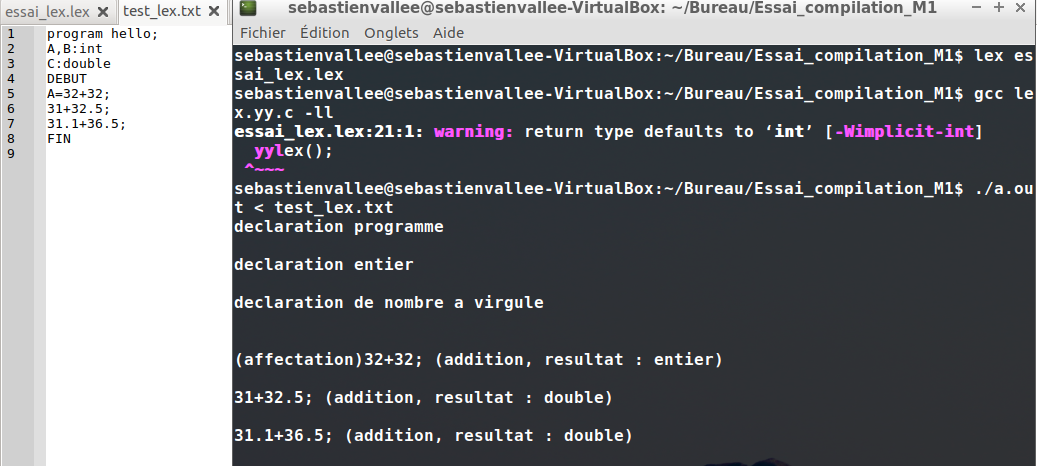
\includegraphics[scale=0.6]{data/lex}}
    \caption{Résultat du code lex}
    \label{fig:lex}
\end{figure}

Sur la figure \href{fig:lex}{1},  on peut voir que le but du programme est de remplacer les lignes du programme du fichier en entrée, par une description des expression qu'il trouve. Par exemple, on peut lire sur la sortie standard que la deuxième ligne du programme est une déclaration d'entier ; ou que l'addition 32+32 est précédé d'une affectation à une variable, tandis que les deux additions suivante non.
Lorsque qu'un mot n'est pas reconnu par Lex, il est par défaut envoyé sur la sortie standard, ce qui n'est pas le cas pour ce mot (le fichier en entrée).

Alors bien que Lex peut offrir des outils puissant, l'analyse de fichiers peut s'avérer assez difficile. On ne peut par exemple, pas savoir si les additions sont bien entre les balises "DEBUT" et "FIN" (sauf en écrivant un code c inutilement compliqué). Nous verrons plus tard qu'un autre outil est plus puissant dans ces cas là.

\section{Yacc}
    Lex et yacc sont des outils similaire : ce sont tous les deux gérateur d’analyseur syntaxique.

Leur fonctionnement est très similaire dans le sens où il permettent d'associer des actions lorsque qu'un mot du texte en entrée est reconnu.

Cependant, le fonctionnement de yacc est légèrement plus puissant. En effet, il permet de fonctionner avec une grammaire.

Le code yacc est divisé en 3 partie que nous allons voir rapidement.

\subsection{première partie}
cette première partie commence par \%\{ et finie par \%\}. Elle permet de définir tous les besoins du code c/c++. C'est à dire la déclaration des variables, des constantes, des fonctions,etc...

\subsection{deuxième partie}
Cette partie contient l'ensemble de la grammaire et des actions qui lui sont associé. C'est dans cette partie que yacc se distingue de Lex.
En effet, là où Lex utilise des définitions régulières et un ensemble de règles, Yacc se contente d'associer à chaque règle d'une grammaire une ou des actions c++.

A l'exécution, cette différence s'exprime par le fait que les règles de Lex sont fixes. Lex va essayer de trouver le mot le plus long qui permet de matcher à une règle. C'est à dire qu'il y à un match pour une seule règle. Une fois le mot trouvé, Lex "oublie" totalement la règle utilisé et passe à la recherche du mot suivant.
Yacc lui permet de remonter les règles et donc d'effectuer plusieurs actions à différents moments sur une même chaîne de caractère. C'est à dire qu'il va se souvenir des règles qu'il traverse.
Ce fonctionnement ressemble fortement à ce que nous avons fais dans le code : parcourir l'arbre de notre grammaire et effectuer des actions en fonction du noeud où nous sommes. Yacc fonctionne exactement pareil.

cette grammaire se définie de la manière suivante : \newline

\begin{tabular}{|c|}
    \hline
        NON\_TERMINAL: expression \\
    \hline
\end{tabular}
\newline

En premier, le non-terminal suivie de deux points. Puis une expression pouvant contenir des non-terminaux, des terminaux ou des symboles spéciaux tel que | pour la règle "ou" des grammaire, etc...

\subsection{troisième partie}
Cette partie est la déclaration des fonctions c++ de la première partie et de la déclaration de la fonction principale du programme.

\subsection{exemple de code Yacc}
Vous pourrez trouvez un exemple de code Yacc dans le répertoire github (qui vous est donné à la fin de ce rendu).
Ce code yacc permet de récupérer des opérations d'additions ou de multiplication entre des entiers (deux,trois, quatre, ...) et d'afficher le resultat dans la sortie standard. Le code est contenue dans le fichier essai\_yacc.yxx.
Celui-ci peut être compilé avec les commande :\newline

\begin{tabular}{|c|}
    \hline
        \$ yacc essai\_yacc.yxx \\
        cela générera un fichier y.tab.c mais qui devra être compilé \\
         avec un compilateur c++ (dû à l'utilisation d'iostream et des cout,cin)\\
    \hline
        \$ g++ y.tab.c \\
        (générera l'exécutable qui peut être lancé avec la commande \$ ./a.out) \\
    \hline
\end{tabular}
\newline

Le résultat du code est le suivant, de la forme " $-->$ resultat\_operation ":
\newline

\begin{figure}[h]
    \centerline{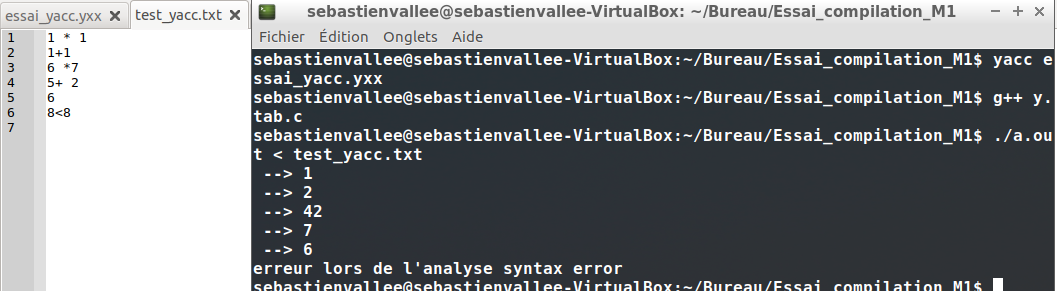
\includegraphics[scale=0.7]{data/yacc}}
    \caption{resultat du code yacc}
    \label{fig:yacc}
\end{figure}

Sur la figure \href{fig:yacc}{2}, on peut voir que le programme s'arrête sur une erreur : la dernière ligne "8 $<$ 8" ne respecte aucune règle donc le mot (tout le fichier) est faux et le programme s'arrête.

\newpage

\section{Conclusion}
Pour conclure, nous pouvons constater qu'il est assez trivial de prendre rapidement en main Lex et Yacc.
\newline
\'A l'aide de Lex et de Yacc, il serait donc possible de créer un compilateur d’un langage relativement simple possédant des fonctionnalités basiques.

\section*{Dépot Github}
Voici le lien de notre dépot github : 
\newline
https://github.com/PineauSullivan/Workspace\_master/tree/master/Compilation/projet/Lex\_et\_yacc

\end{document}
